\glsreset{clf}\glsreset{cbf}
Based on \citep{bib:artstein}, which founded \gls{clf}s, a \gls{cbf} can be created \citep{bib:org_control}. With a system $\dot{x}=f(x)+g(x)u$, a \gls{cbf} exist if the below constraints are fulfilled:
\begin{flalign}
& x\in \mathcal{X}_u \hspace{0.3cm} \Rightarrow \hspace{0.3cm} B(x) > 0  \label{req1} \\
& L_gB(x) = 0 \hspace{0.3cm} \Rightarrow \hspace{0.3cm} L_fB(x) < 0 \label{req2} \\
& \{ x \in \mathcal{X} | B(x) \leq 0 \} \neq \emptyset \label{req3}
\end{flalign}
\vspace{-0.8cm}
\begin{longtable}{p{.9\textwidth} p{.1\textwidth} p{.1\textwidth}} 
Where  & & \\
$B(x)$ is a control barrier function & [$\cdot$] \\ 
$L_fB(x)$ is the Lie derivative of $B(x)$ along the vector field  $f(x)$, i.e. $\frac{\partial B(x)}{\partial x}f(x)$ & [$\cdot$] \\ 
$L_fB(x)$ is the Lie derivative of $B(x)$ along the vector field  $g(x)$, i.e. $\frac{\partial B(x)}{\partial x}g(x)$ & [$\cdot$] 
\end{longtable}
\vspace*{-0.2cm}
Taking a look at \autoref{req1} it states essentially the same as \autoref{cer2}, i.e. the unsafe area exist whenever $B(x)>0$. This makes it possible to design an unsafe region. \Autoref{req2} put forth the requirement that the gradient along the vector field $f(x)$ must point away from the barrier extremities whenever the input is with no significance (except for the critical point). \Autoref{req3} simply states that the safe area must contain some states as control otherwise is impossible.
\section{Safe Controller for Instrument Slide}
The slide movement is visualized in \autoref{fig:slidefig} and an overview of terms used in this section is found in \autoref{fig:safe:overview}.
\begin{figure}[H]
    \centering
    \begin{minipage}{.5\textwidth}
        \centering
        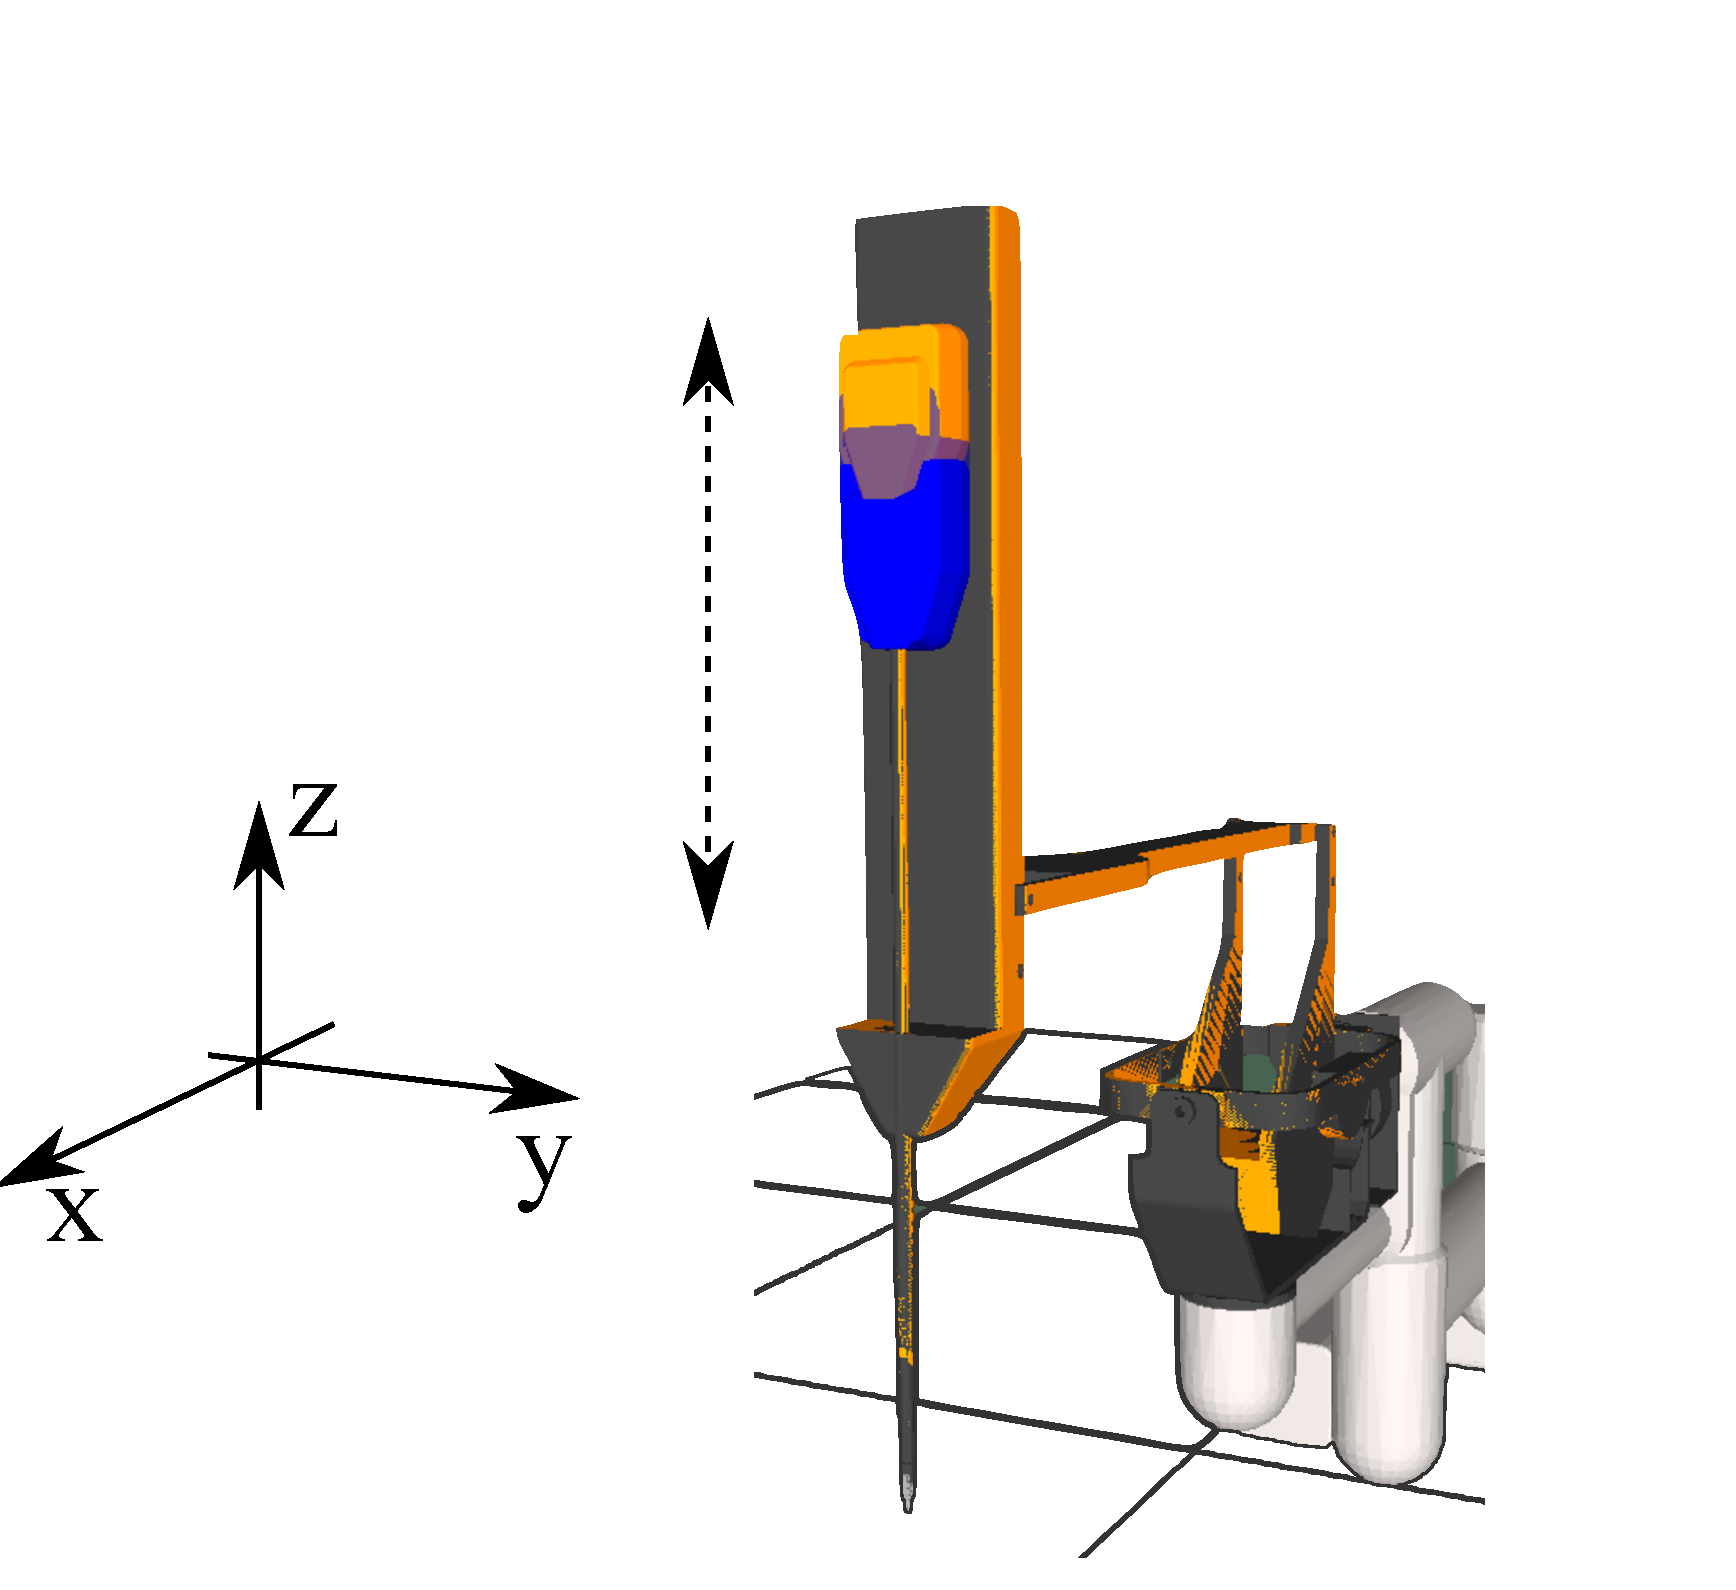
\includegraphics[width=0.73\linewidth]{slidemovefigure.pdf}
        \caption{Illustration of slide movement.}
        \label{fig:slidefig}
    \end{minipage}%
    \begin{minipage}{0.5\textwidth}
        \centering
        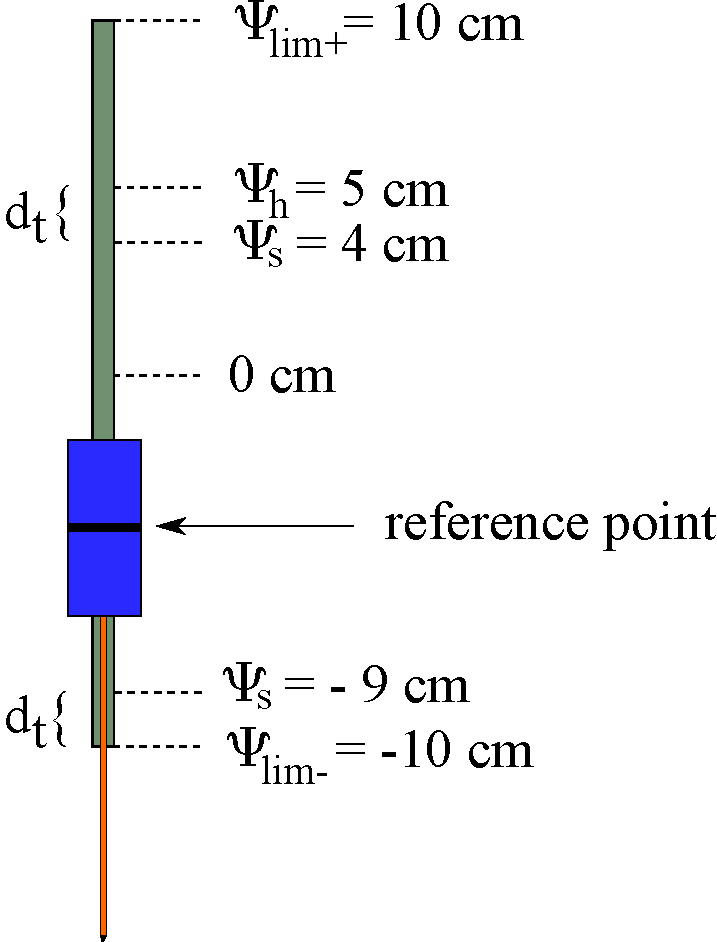
\includegraphics[width=0.7\linewidth]{slide_overview.pdf}
        \caption{Boundaries used in this section.}
        \label{fig:safe:overview}
    \end{minipage}
\end{figure}
A system model is required before any controller design may be initiated.
%\hspace{1cm }\texttt{rostopic echo joint\_states/position[6]} \hspace{0.2cm} {\color{blue}{\# Be sure to have the ROS environment correctly configured according to \autoref{app:ros}}}
\section{Modelling of Slide Movement}
 To obtain a model, a step response will be performed on the slide movement. The slide position can be measured by subscribing to the \texttt{joint\_state} topic in \gls{ros}. The experiment is described in further details in \autoref{app:meas}. To model the system, a step is added to the system. The step response is plotted in \autoref{fig:stepresponseslide}.
\begin{figure}[H]
\center
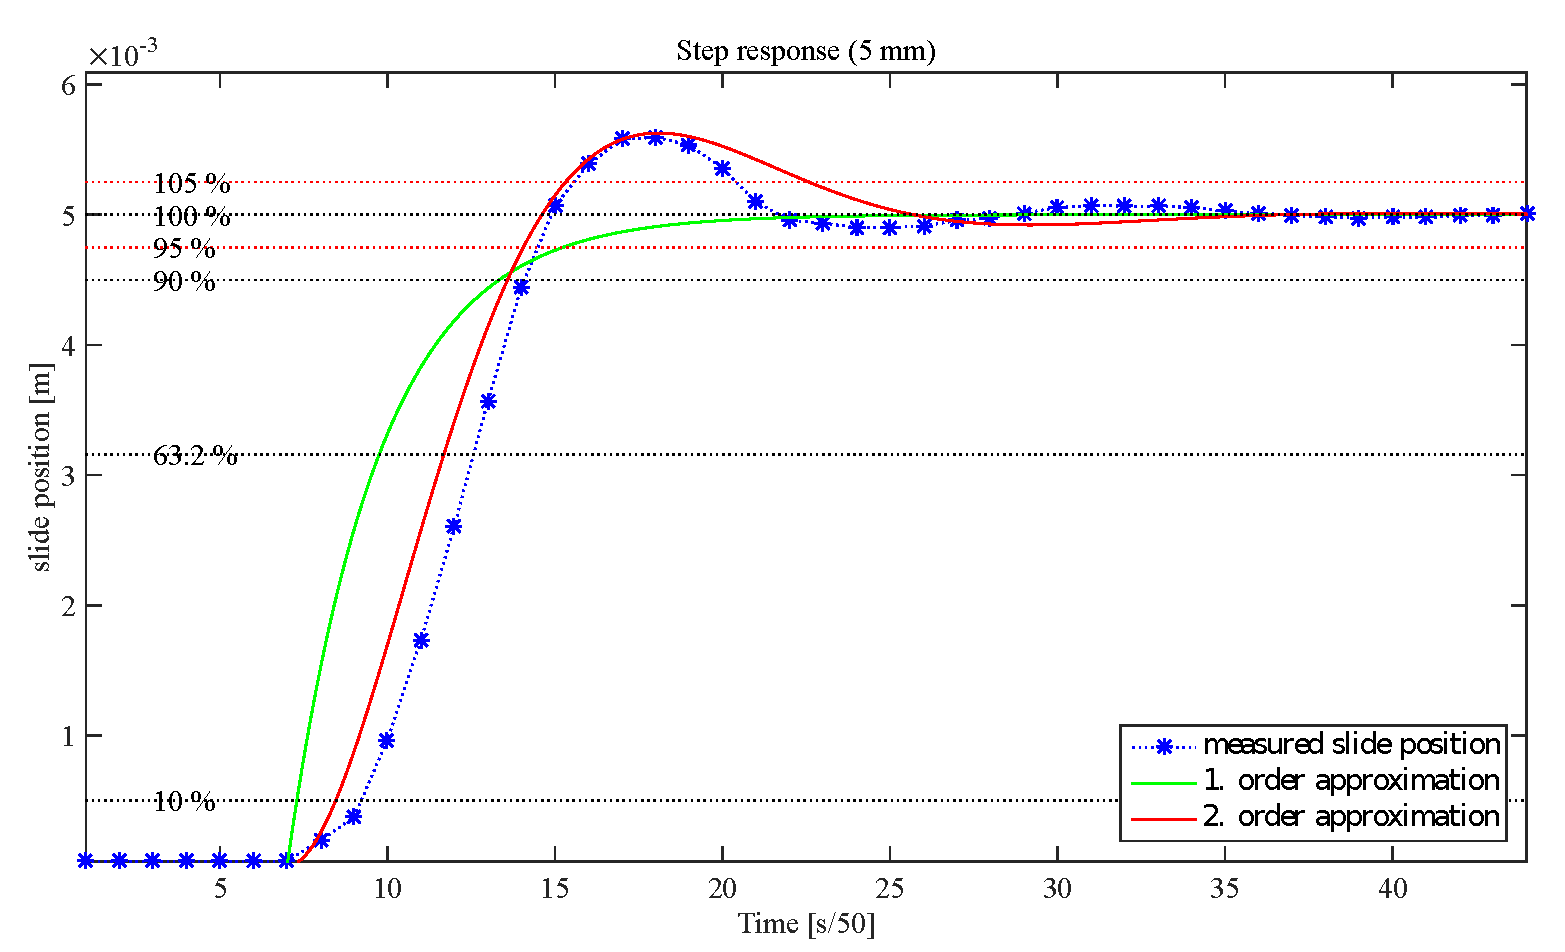
\includegraphics[scale=0.5]{step_slide.pdf}
\caption{Step response from 0\,mm to 5\,mm. Plot details and measurements can be found in \autoref{app:cd} as \texttt{matlab\_scripts/slide\_step/plot\_slide\_pos.m}}
\label{fig:stepresponseslide}
\end{figure}
It is clear that this could be well approximated with an underdamped second order model (complex roots), however for initial simplicity and because modelling is not a focus point in this thesis, merely a simple model of the slide movement is used (it shall later be approximated to a second order model). Therefore, with some good will, it is approximated to a linear first order system with a dominating time constant \gls{taus}: 
\begin{flalign*}
& Y(s) = \dfrac{1}{\tau_s s + 1}U(s) =  \dfrac{1/\tau_s}{s + 1/\tau_s}\,U(s) = (s+1/\tau_s)^{-1}\,1/\tau_s\,U(s) \kk  \overset{\overset{Y(s)=(C(sI-A)^{-1}B+D)U(s)}{\longrightarrow}}{\scriptsize \text{compare to obtain SS form}}  \\ 
& \dot{x} = \underbrace{-\tau_s^{-1}\,x}_{f_s(x)} + \underbrace{\tau_s^{-1}}_{g_s(x)} u
\end{flalign*}
Thus the system matrix $A$ and the input matrix $B$ can be seen easily. For the sake of generalization, they are named $f_s$ and $g_s$, i.e.:
\begin{flalign*}
f_s(x) = -\tau^{-1}x \kk \wedge \kk g_s(x) = \tau_s^{-1}
\end{flalign*}
A suitable time constant $\tau_s$ can be read from \autoref{fig:stepresponseslide} to:
\begin{flalign*}
\tau_s = 55\, \text{ms}
\end{flalign*} 
\section{Construction of CBF}
To illustrate the usefulness of \gls{cbf}s, a palpable example hereof will be created with direct application to the Da Vinci robot. This example does not directly constitute application to a patient but favour the theory in a neat and comprehensible sense and secure a way to visually and physically verify the method.

Consider the state intervals defined in \autoref{tab:intervals}.
\begin{table}[H]
	\begin{tabularx}{\textwidth}{X X X }
\rowcolor{HeaderBlue} 
$\mathcal{X}$ & $\mathcal{X}_u$  & $\mathcal{X}_0$ \\
$x \in \{[\Lambda_{s+}:\Lambda_\text{lim+}],[\Lambda_\text{lim-}:\Lambda_{s-}]\}$  & $x \in \{[\Lambda_{h+}:\Lambda_\text{lim+}],[\Lambda_\text{lim-}:\Lambda_{h-}]\} $ & $x \in \{[\Lambda_{s+}:\Lambda_{lim+}],[\Lambda_\text{lim-}:\Lambda_{s-}]\}$  \\
\end{tabularx}
\caption{Global state intervals where: $\Lambda_\text{lim}$ is the physical slide limit ($\pm$0.1\,m), $\Lambda_s$ is a soft limit denoting a transition area and $\Lambda_h$ is a hard limit where a trajectory at all cost can not cross. The interval $x \in [\Lambda_{s-}:\Lambda_{s+}]$ is safe thus any control law can be used in that area.}
\label{tab:intervals}
\end{table}
A parabola is now introduced as \gls{cbf}. A coordinate shift is performed such that the slide movement occurs along the $x$-axis instead of the $z$-axis. 
\begin{flalign*}
B(x) = ax^2+bx+c \kk \Rightarrow \kk L_fB(x) = \dfrac{d}{dx}B(x)f_s(x) = (2ax+b)(-\tau^{-1}x) = -2\tau^{-1}ax^2-\tau^{-1}bx
\end{flalign*}
\Autoref{req2} put forth the demand that $L_fB(x)<0$ when $L_gB(x) = 0$ as the input in that case will be insignificant. Ensuring that $L_fB(x)<0$ in the area $x \in [\Lambda_s:\Lambda_h]$ is therefore indeed sufficient. Analysis of $L_fB(x)$ shall reveal when $L_fB(x)>0$, i.e. to ensure the demand below:
\begin{flalign*}
L_fB(x) \ngtr 0\hspace{0.3cm}\forall\hspace{0.3cm} x \in [\Lambda_s:\Lambda_h]
\end{flalign*}
Thus the analysis is performed:
\begin{flalign}
L_fB(x) < 0 \kk \Leftrightarrow \kk -2\tau^{-1}ax^2-\tau^{-1}bx < 0
\label{eq:analysis}
\end{flalign}
The coefficients $a$ and $b$ must be found. By studying $x>0$ it can from \autoref{eq:analysis} be seen that:
\begin{flalign*}
\forall \mm \{ a > 0 \mm  \wedge \mm b > 0 \} \mm \Rightarrow \mm L_fB(x) < 0 \mm \forall \mm  x > 0
\end{flalign*}
The scenario changes when $x<0$. Preserving that $a>0$ and $b>0$, the analysis below put forth constraints to the x.
\begin{flalign}
&L_fB(x) = 0 \kk \Leftrightarrow \kk  -2\tau^{-1}ax^2-\tau^{-1}bx = 0 \nonumber
 \\  &-2ax^2-bx = 0 \mm \Rightarrow \mm x = 
\begin{cases}
  \frac{-b}{2a} \\
   0,             
\end{cases}
\label{eq:interval1}
\end{flalign}
Thus, $B(x)$ is not a valid barrier function within the interval:
\begin{flalign}
B(x) \hspace{0.15cm} \text{invalid:} \mm  x \in \left[ \frac{-b}{2a}:0 \right] \mm \text{if} \mm L_gB(x) = 0
\label{eq:interval}
\end{flalign}
Three equations with three unknowns can be outlined to fulfil the initial demand in figure ??.
\begin{flalign*}
 \left.
 \begin{aligned}
a\,\Lambda_h^2 + b\,\Lambda_h + c = 0 \\
a\,(-\Lambda_\text{lim})^2 + b\,(-\Lambda_\text{lim})^2 + c = 0 \\
a\left( \frac{-\Lambda_\text{lim}+\Lambda_h}{2}\right)^2 + b\left(\frac{-\Lambda_\text{lim}+\Lambda_h}{2}\right) + c = \underbrace{-0.025}_\text{any constant $<0$} 
\end{aligned}
\mm \right\}
 \qquad \begin{matrix}
 a &= \,\,\,\,\,\,\,\,1.7778 \\ b &= \,\,\,\,\,\,\,\,0.0889 \\ c &= -0.0089
 \end{matrix}
\end{flalign*}
The interval where $B(x)$ is invalid can thereby be found from \autoref{eq:interval}:
\begin{flalign*}
B(x) \hspace{0.15cm} \text{invalid:} \mm  x \in [-0.0250:0]
\end{flalign*}
This is indifferent as $\mathcal{X}  \notin [\Lambda_{s-}:\Lambda_{s+}]$. Thus the barrier function is a valid \gls{cbf}. It is plotted in \autoref{fig:barrierfunction}
\begin{figure}[H]
\center
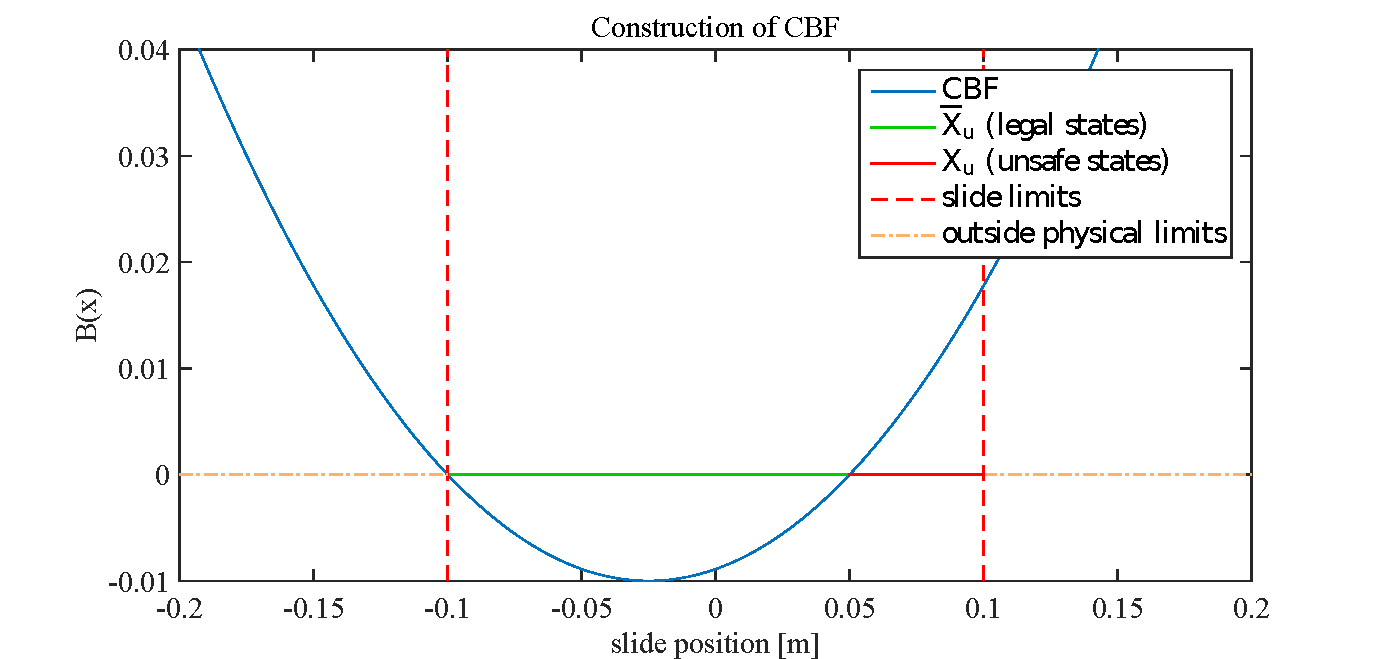
\includegraphics[scale=0.5]{parabel_1.pdf}
\caption{Barrier function along with the $\mathcal{X}_u$ and $\mathcal{X}_u^c$. Plot details and MATLAB script can be found in ????}
\label{fig:barrierfunction}
\end{figure}
\section{Controller Design}
A control laws is now introduced:
\begin{flalign*}
u(x) =
\begin{cases}
	\bar{N}\,x_\text{ref} - K\,x \kk &\text{if \mm $x \in [\Lambda_{s-}:\Lambda_{s+}]$}\\
	 k_0(x)  \kk &\text{if \mm $x \in [\Lambda_{s+}:\Lambda_{h+}] \mm \wedge \mm x \in [\Lambda_{h-}:\Lambda_{s-}]$}
\end{cases}
\end{flalign*}
This can be refined with a parameter $\sigma(x)$ such that the shift between the two control laws is not instantaneous \citep{bib:org_control}. Consider the control law below:
\begin{flalign*}
u(x) = \sigma(x)k_0(x)+(1-\sigma(x))\tilde{u}(x) = \sigma(x)k_0(x)+(1-\sigma(x))(\bar{N} \cdot x_\text{ref}-Kx) 
\end{flalign*}
\vspace{-0.8cm}
\begin{longtable}{p{.9\textwidth} p{.1\textwidth} p{.1\textwidth}} 
Where  & & \\
$u(x)$ is a control signal where safety is ensured  & [$\cdot$] \\
$\tilde{u}(x)$ is a control signal to the linear state space system such that $\tilde{u}=\bar{N}\cdot x_\text{ref}-Kx$ & [$\cdot$] \\ 
$k_0(x)$ is a control law that guarantees safety & [$\cdot$] \\ 
$\sigma(x)$ is a parameter that founds a linear combination between the two control inputs & [$\cdot$] \\ 
$K$ is a constant feedback matrix in $\mathbb{R}^{1 \times 1}$ & [$\cdot$] 
\end{longtable}
\vspace*{-0.2cm}
The control law is thereby a linear combination of two controllers. It is noted that:
\begin{flalign*}
\sigma(x) = 
\begin{cases}
0 \mm &\Rightarrow \mm \text{Pure control by pole placement, i.e. $u(x) = \tilde{u}(x) =  \bar{N}\cdot x_\text{ref}-Kx$ } \\
1 \mm &\Rightarrow \mm \text{Pure control for safety i.e. $u(x) = k_0(x)$ } \\
]0:1[ \mm &\Rightarrow \mm \text{A linear combination of the two control signals $u(x)$ and $\tilde{u}(x)$}
\end{cases}
\end{flalign*}
A block diagram is depicted in \autoref{fig:controlsystem}.
\begin{figure}[H]
	\center
		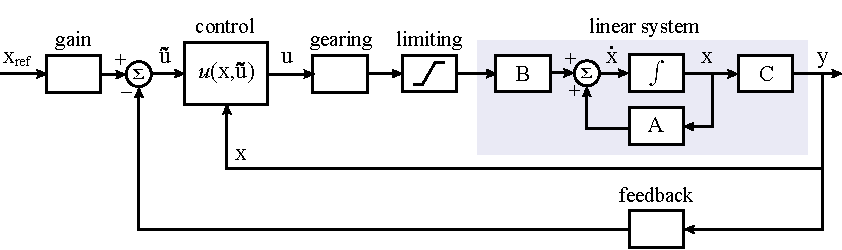
\includegraphics[scale=1]{control_system.pdf}
	\caption{Block diagram of the control system for slide position. MATLAB implementation is found in \autoref{app:slide_implement_1}.}
	\label{fig:controlsystem}
\end{figure}
\subsection{Construction of $k_0$}
The control law ensuring safety can be found as \citep{bib:org_control}:
\begin{flalign}
k_0(x) = \begin{cases}
-\dfrac{L_fB(x)+ \sqrt{(L_fB(x))^2 + \kappa^2(L_gB(x))^TL_gB(x)}}{(L_gB(x))^TL_gB(x)}L_gB(x) &\text{if} \mm L_gB(x) \neq 0 \\
0  &\text{if} \mm L_gB(x) = 0
\end{cases}
\label{eq:control_law}
\end{flalign}
$\kappa$ is a design variable. High values of $\kappa$ implies increased aggressiveness. \Autoref{eq:control_law} ensures indeed safety for the closed loop system $\dot{x} = f_s(x)+g_s(x)k_0(x)$. This is easily proven as:
\begin{flalign*}
L_{f_{cl}}B(x) = L_fB(x) + L_gB(x)k_0(x)
\end{flalign*}
For $L_gB(x) \neq 0:$
\begin{flalign*}
L_{f_{cl}}B(x) &= L_fB(x) + L_gB(x) \left( -\dfrac{L_fB(x)+ \sqrt{(L_fB(x))^2 + \kappa^2(L_gB(x))^TL_gB(x)}}{(L_gB(x))^TL_gB(x)}L_gB(x) \right)  \\
&= L_fB(x) - (L_gB(x))^TL_gB(x) \dfrac{L_fB(x) - \sqrt{(L_fB(x))^2 + \kappa^2(L_gB(x))^TL_gB(x)}}{(L_gB(x))^TL_gB(x)}   \\ 
&= L_fB(x) - L_fB(x) - \sqrt{(L_fB(x))^2 + \kappa^2(L_gB(x))^TL_gB(x)} \\
&= - \sqrt{(L_fB(x))^2 + \kappa^2(L_gB(x))^TL_gB(x)} \mm \leq 0 \mm \forall \mm x
\end{flalign*}
As all terms within the square root are squared, no imaginary numbers occur, as a result $L_{f_{cl}}B(x) \leq 0$ 

According to \autoref{eq:control_law}, when $L_gB(x) = 0$:
\begin{flalign*}
L_{f_{cl}}B(x) = L_fB(x) + L_gB(x)\cdot 0 = L_fB(x)
\end{flalign*}
As $L_fB(x)$ is constructed such that $L_gB(x) = 0 \hspace{0.15cm} \Rightarrow \hspace{0.15cm} L_fB(x) < 0 $. 
\subsection{Construction of $K$ and $\bar{N}$}
The system is approximated to a linear system on the form $\dot{x}=Ax+Bu$, thus pole placement can be used. No constraints to the constant feedback matrix $K$ will be outlined except stability. It will therefore be determined from the pole placement method where a closed loop pole that is ten times faster than the open loop pole will be placed. Ackermann's formula can be used \citep{bib:acker}:
\begin{enumerate}
\item Identify the desired closed loop polynomial on as $A_{cl}(s) = s^n + a_{n-1}s^{n-1}  +  \cdots + a_ {c1}s + a_{c0}$: 
\begin{flalign*}
A_{cl}(s) = s + 10\,\tau^{-1}
\end{flalign*}
\item Identify the open loop polynomial as $A_{cl}(s) = s^n + a_{c(n-1)}s^{n-1} +  \cdots + a_1s + a_0$: 
\begin{flalign*}
A_{ol}(s) = \lambda + \tau^{-1}
\end{flalign*}
\item Compute the feedback matrix in controllable canonical form:
\begin{flalign*}
 \bar{K}^T = \begin{bmatrix}
 \bar{k_1} \\
 \vdots \\
 \bar{k_n}
 \end{bmatrix} = \begin{bmatrix}
 a_{c0} - a_0 \\
 \vdots \\
 a_{c(n-1)} - a_{n-1}
 \end{bmatrix} \kk \Rightarrow  \kk \bar{K}^T = 10\,\tau^{-1} - \tau^{-1} = 9\,\tau^{-1}
\end{flalign*}
\item Compute the similarity transform $Q$ recursively as:\\ 
\begin{minipage}[t]{0.3\textwidth}
\begin{flalign*}
&Q = \begin{bmatrix}
q_1 & q_2 & \cdots & q_n
\end{bmatrix} \\
&\text{where:}\\
&\kk q_n = B \\
&\kk q_{j-1} = A\,q_j + a_{j-1}B\\
{\color{white}{white}}\hspace{-0.5cm}
\end{flalign*}
\end{minipage}
\begin{minipage}[t]{0.1\textwidth}
\begin{flalign*}
\Rightarrow
\end{flalign*}
\end{minipage}
\begin{minipage}[t]{0.2\textwidth}
\begin{flalign*}
Q = \tau^{-1}
\end{flalign*}
\end{minipage}
\item Compute the feedback matrix as:
\begin{flalign*}
K = \bar{K}\,Q^{-1} = 9\,\tau^{-1}\dfrac{1}{\tau^{-1}} = 9
\end{flalign*}
\end{enumerate}
The constant feedback matrix, $\bar{N}$, can be computed as \citep{bib:Nbar}:
\begin{flalign*}
\bar{N} = - \left( C\,A_{cl}^{-1}\,B \right)^{-1} =  - \left( C\,(A-B\,K)^{-1}\,B \right)^{-1} = 10
\end{flalign*}
\section{Simulation results}
